\documentclass{beamer}

\usepackage{fontspec} 
% \usepackage{lsp-makros}
\useoutertheme{lsp}

\usepackage{lsptitle}

\def\two@digits#1{\ifnum#1<10 0\fi\number#1}
\def\mytoday{\two@digits{\number\day}.\two@digits{\number\month}.\number\year}


\usepackage{xspace,multicol}
\newcommand{\latex}{\LaTeX\xspace}
\usepackage{tikz}


\newcounter{lastpagemainpart}
\footnotesep0pt
\renewcommand{\footnoterule}{}
\usefootnotetemplate{
  \noindent
  \insertfootnotemark\insertfootnotetext}

\let\beamerfn=\footnote
\renewcommand{\footnote}[1]{%
\let\oldfnsize=\footnotesize%
\let\footnotesize=\tiny%
\beamerfn<\thebeamerpauses->{#1}%
\let\footnotesize=\oldfnsize}


\date{\today}

\usepackage{eurosym}  
 
\renewcommand{\centerline}[1]{\hfill#1\hfill\hfill\mbox{}}


\title{Production}
% \institute{FU Berlin}
\author[LangSci]{Language Science Press}



\begin{document}
\lspbeamertitle

\frame{
\frametitle{Routes to the book}
%   \includegraphics[height=.2\textheight]{./path/to/graphicsfile}
  \begin{enumerate}
    \item  native LaTeX route
    \item Word/LibreOffice route
  \end{enumerate}
}

\section{Native LaTeX route}
\frame{
\frametitle{LaTeX route}
  \begin{itemize}
    \item use our class \texttt{langscibook}, available from CTAN
    \item use our templates
    \item get in touch early
    \item use sanity checker
    \item we will eventually see your code anyway. There is no reason to hide it, so you might as well show it to us early on (even before submission)
  \end{itemize}
}

\frame{
\frametitle{Sanity checker}
\url{http://www.glottotopia.org/doc2tex/doc2tex}

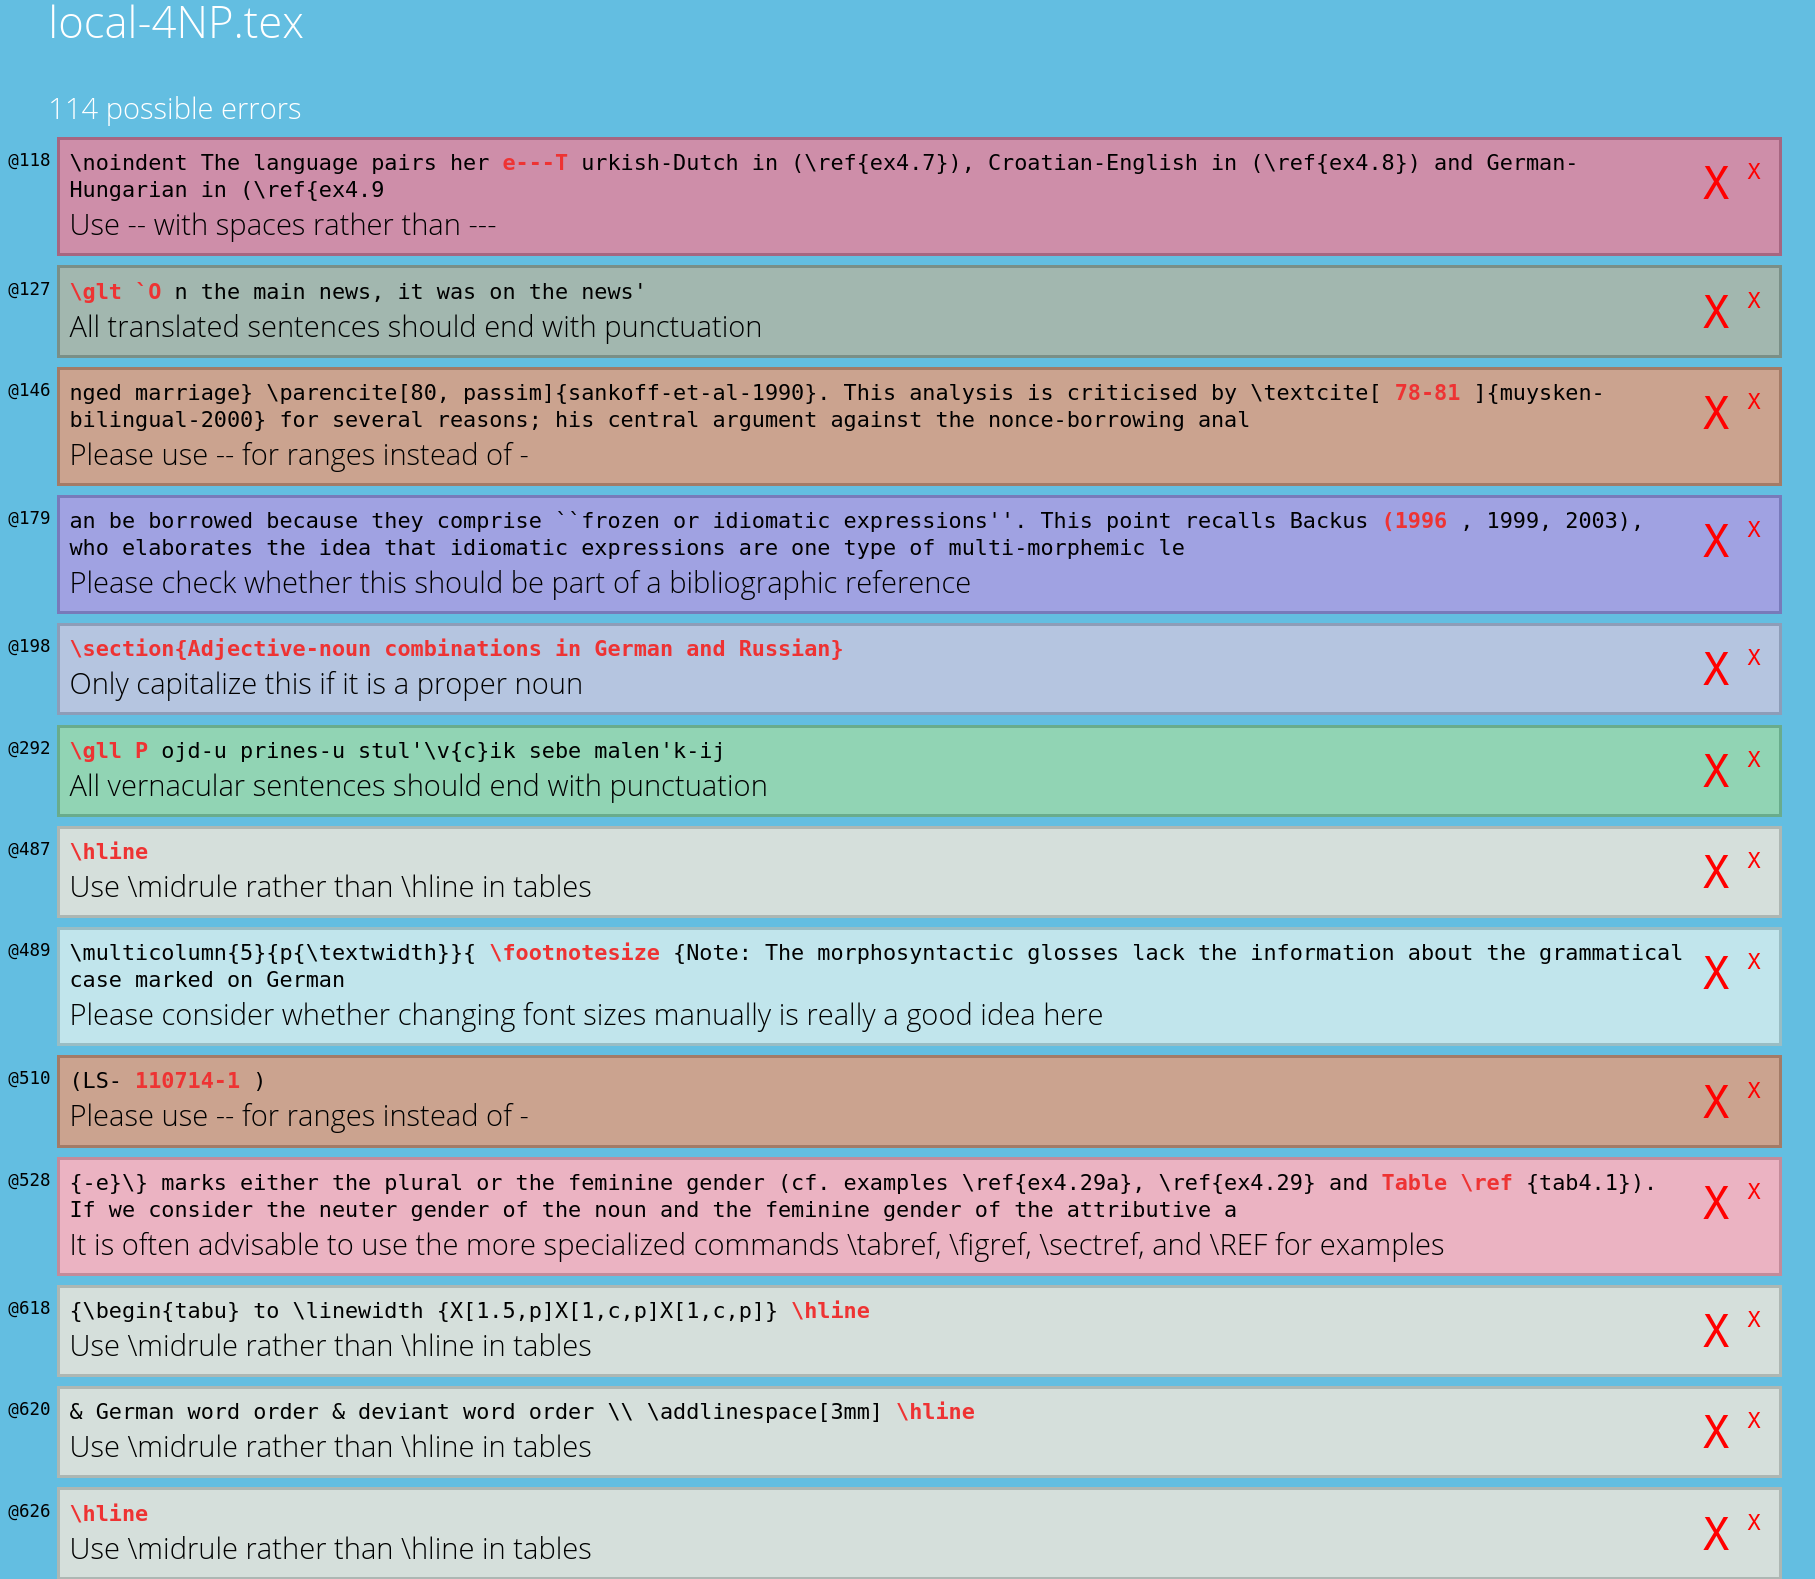
\includegraphics[height=\textheight]{sanitycheck.png}
}


\section[MS Word/LibreOffice]{MS Word/LibreOffice route}
\subsection{Monograph}

\frame{
\frametitle{MS Word/LibreOffice route\newline Monographs}
  \begin{itemize}
    \item     use a citation manager\pause
    \item \large    use a citation manager\pause
    \item \Large    use a citation manager\pause
    \item \LARGE    use a citation manager\pause
    \item \huge \color{red}   !!use a citation manager!!
  \end{itemize}
}

\frame{
\frametitle{More hints}
  \begin{itemize}
    \item     use a citation manager
    \item do not put examples in tables
    \item     use a citation manager
  \end{itemize}
}

 \frame{
\frametitle{Monograph conversion}
%   \includegraphics[height=.2\textheight]{./path/to/graphicsfile}
  \begin{itemize}
    \item   rough conversion done by LangSci
    \begin{enumerate}
      \item   \textbf{Option 1}: conversion before revisions
      \begin{itemize}
        \item
      might cause delays, but only need to touch every chapter once
      \end{itemize}
      \item  \textbf{Option 2}: after revisions
      \begin{itemize}
        \item       will have to touch each chapter twice: once for content, once for postprocessing
      \end{itemize}
    \end{enumerate}
    \item   Overleaf link provided to author for postprocessing
  \end{itemize}
}


\frame{
\frametitle{Overleaf: postprocessing}
\hspace*{-.5cm}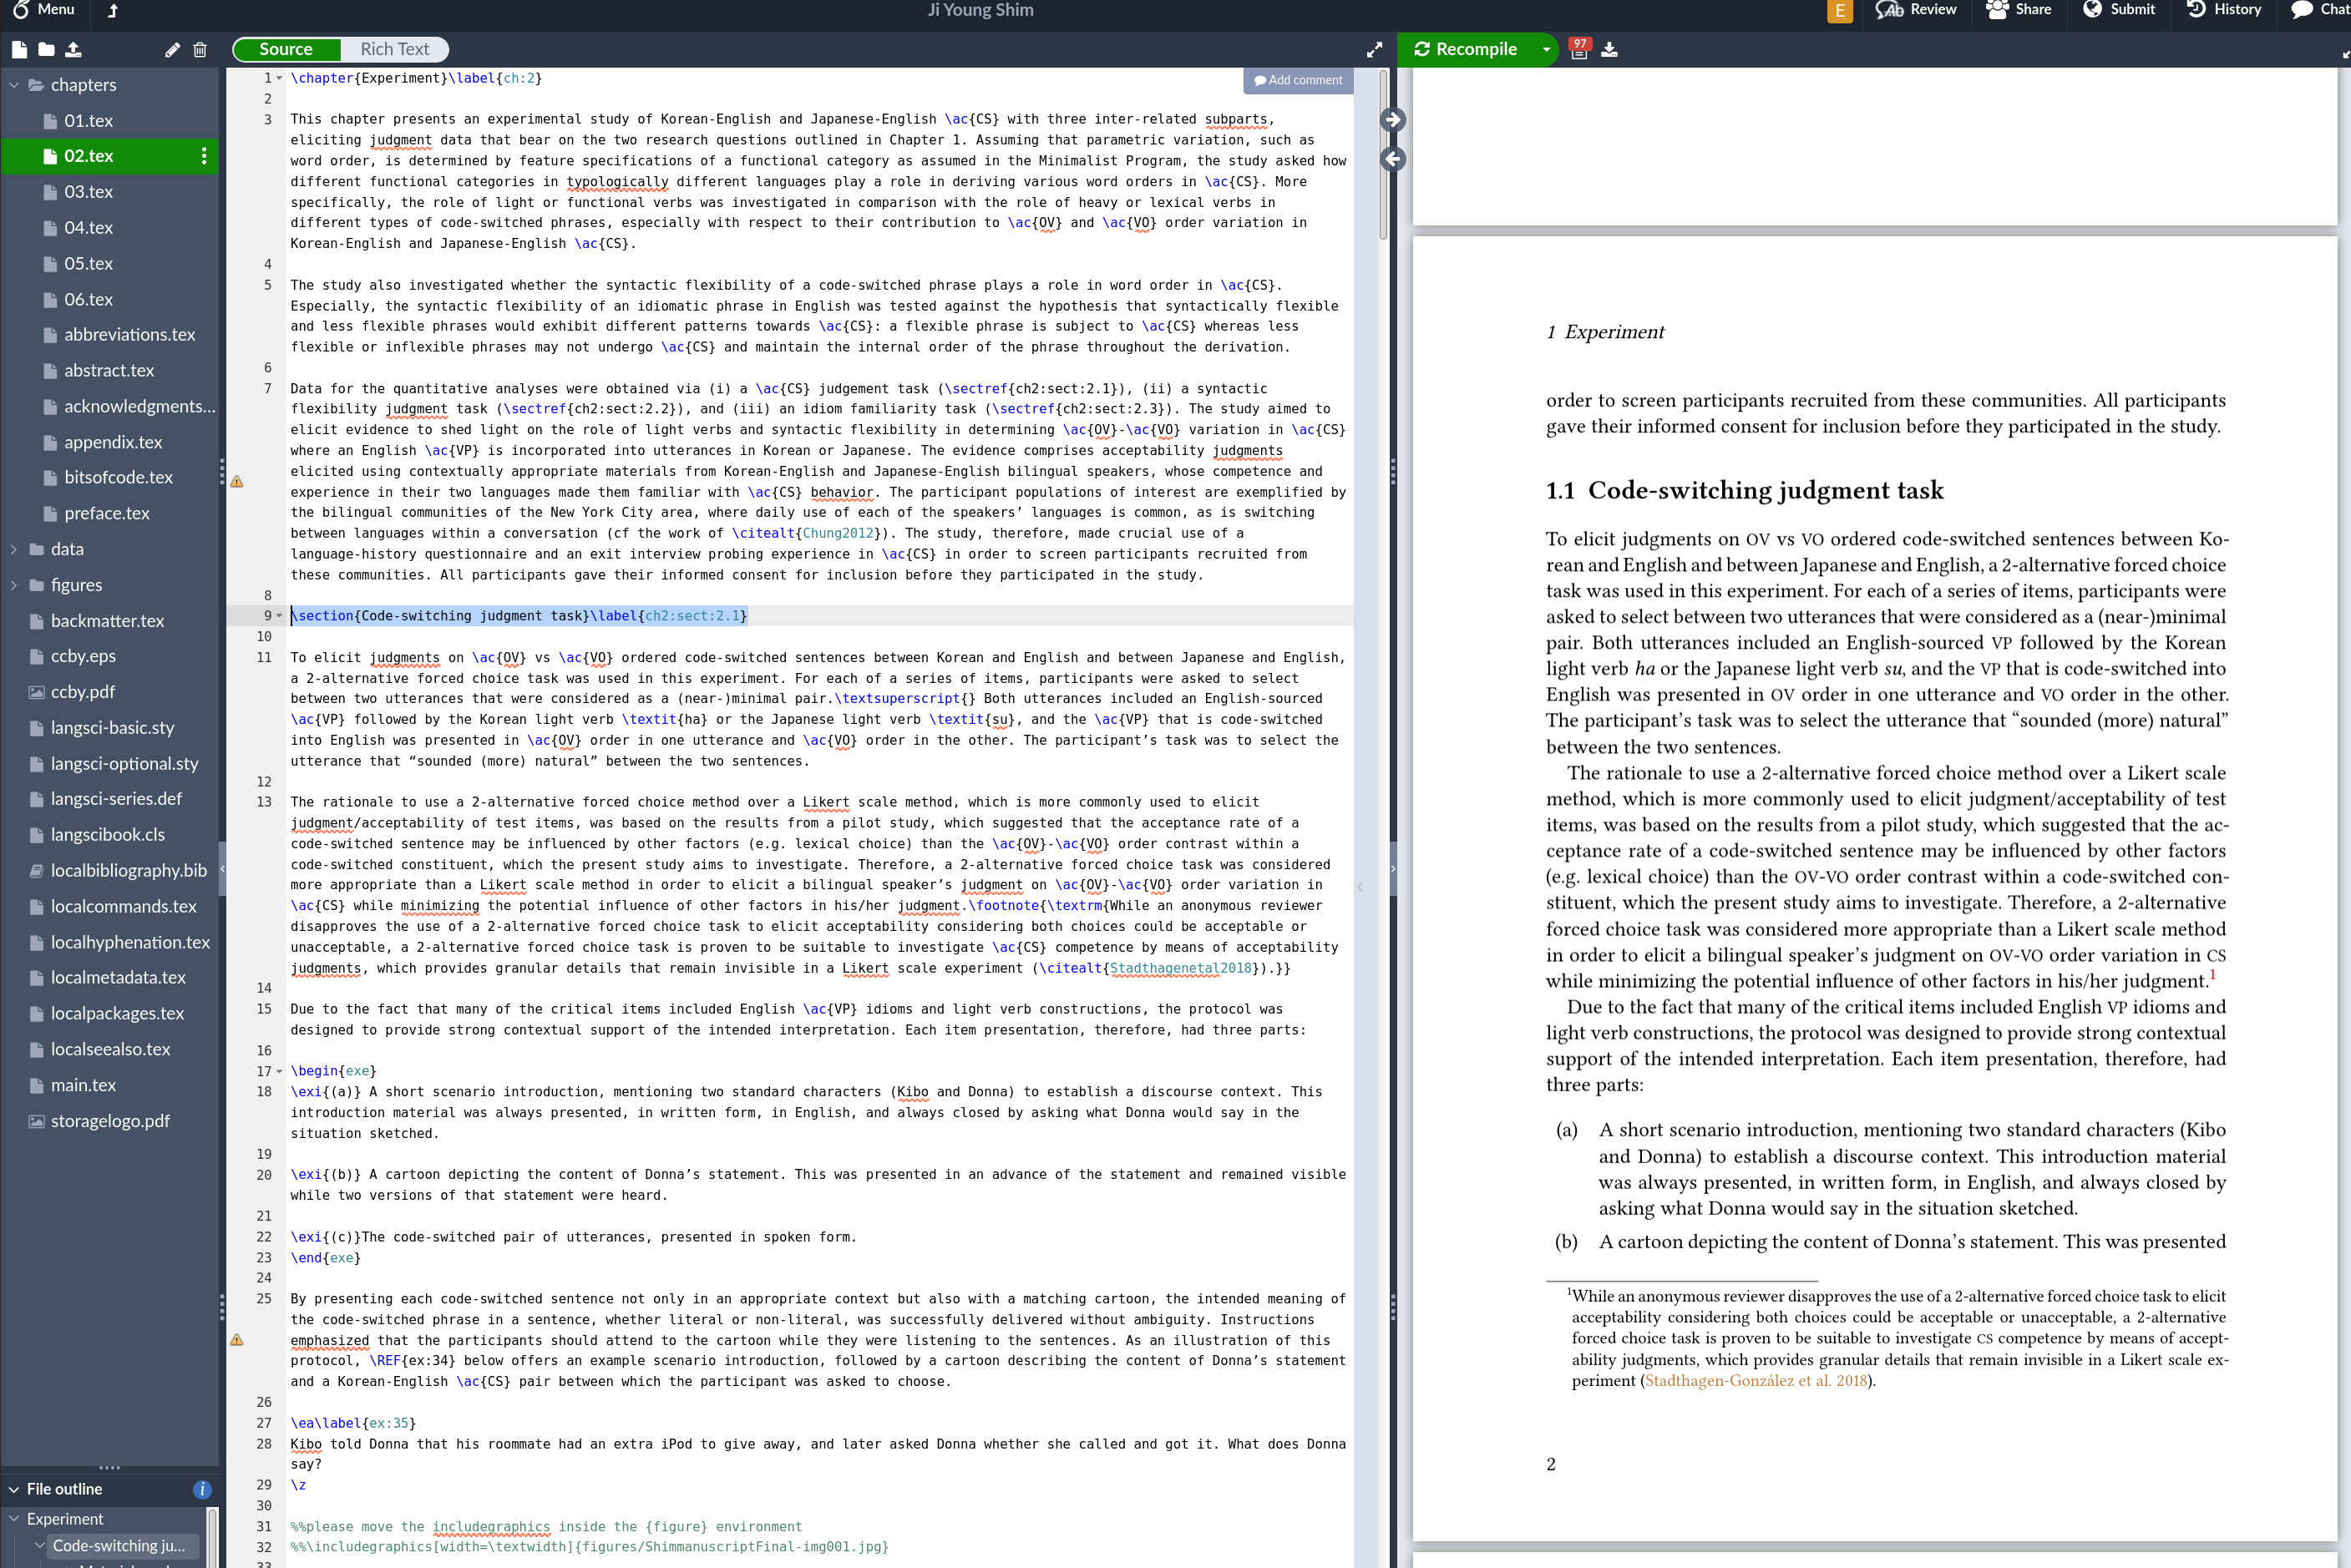
\includegraphics[width=1.1\textwidth]{overleaf.png}
}

\frame{
\frametitle{Overleaf: rough edges}
\hspace*{-.5cm}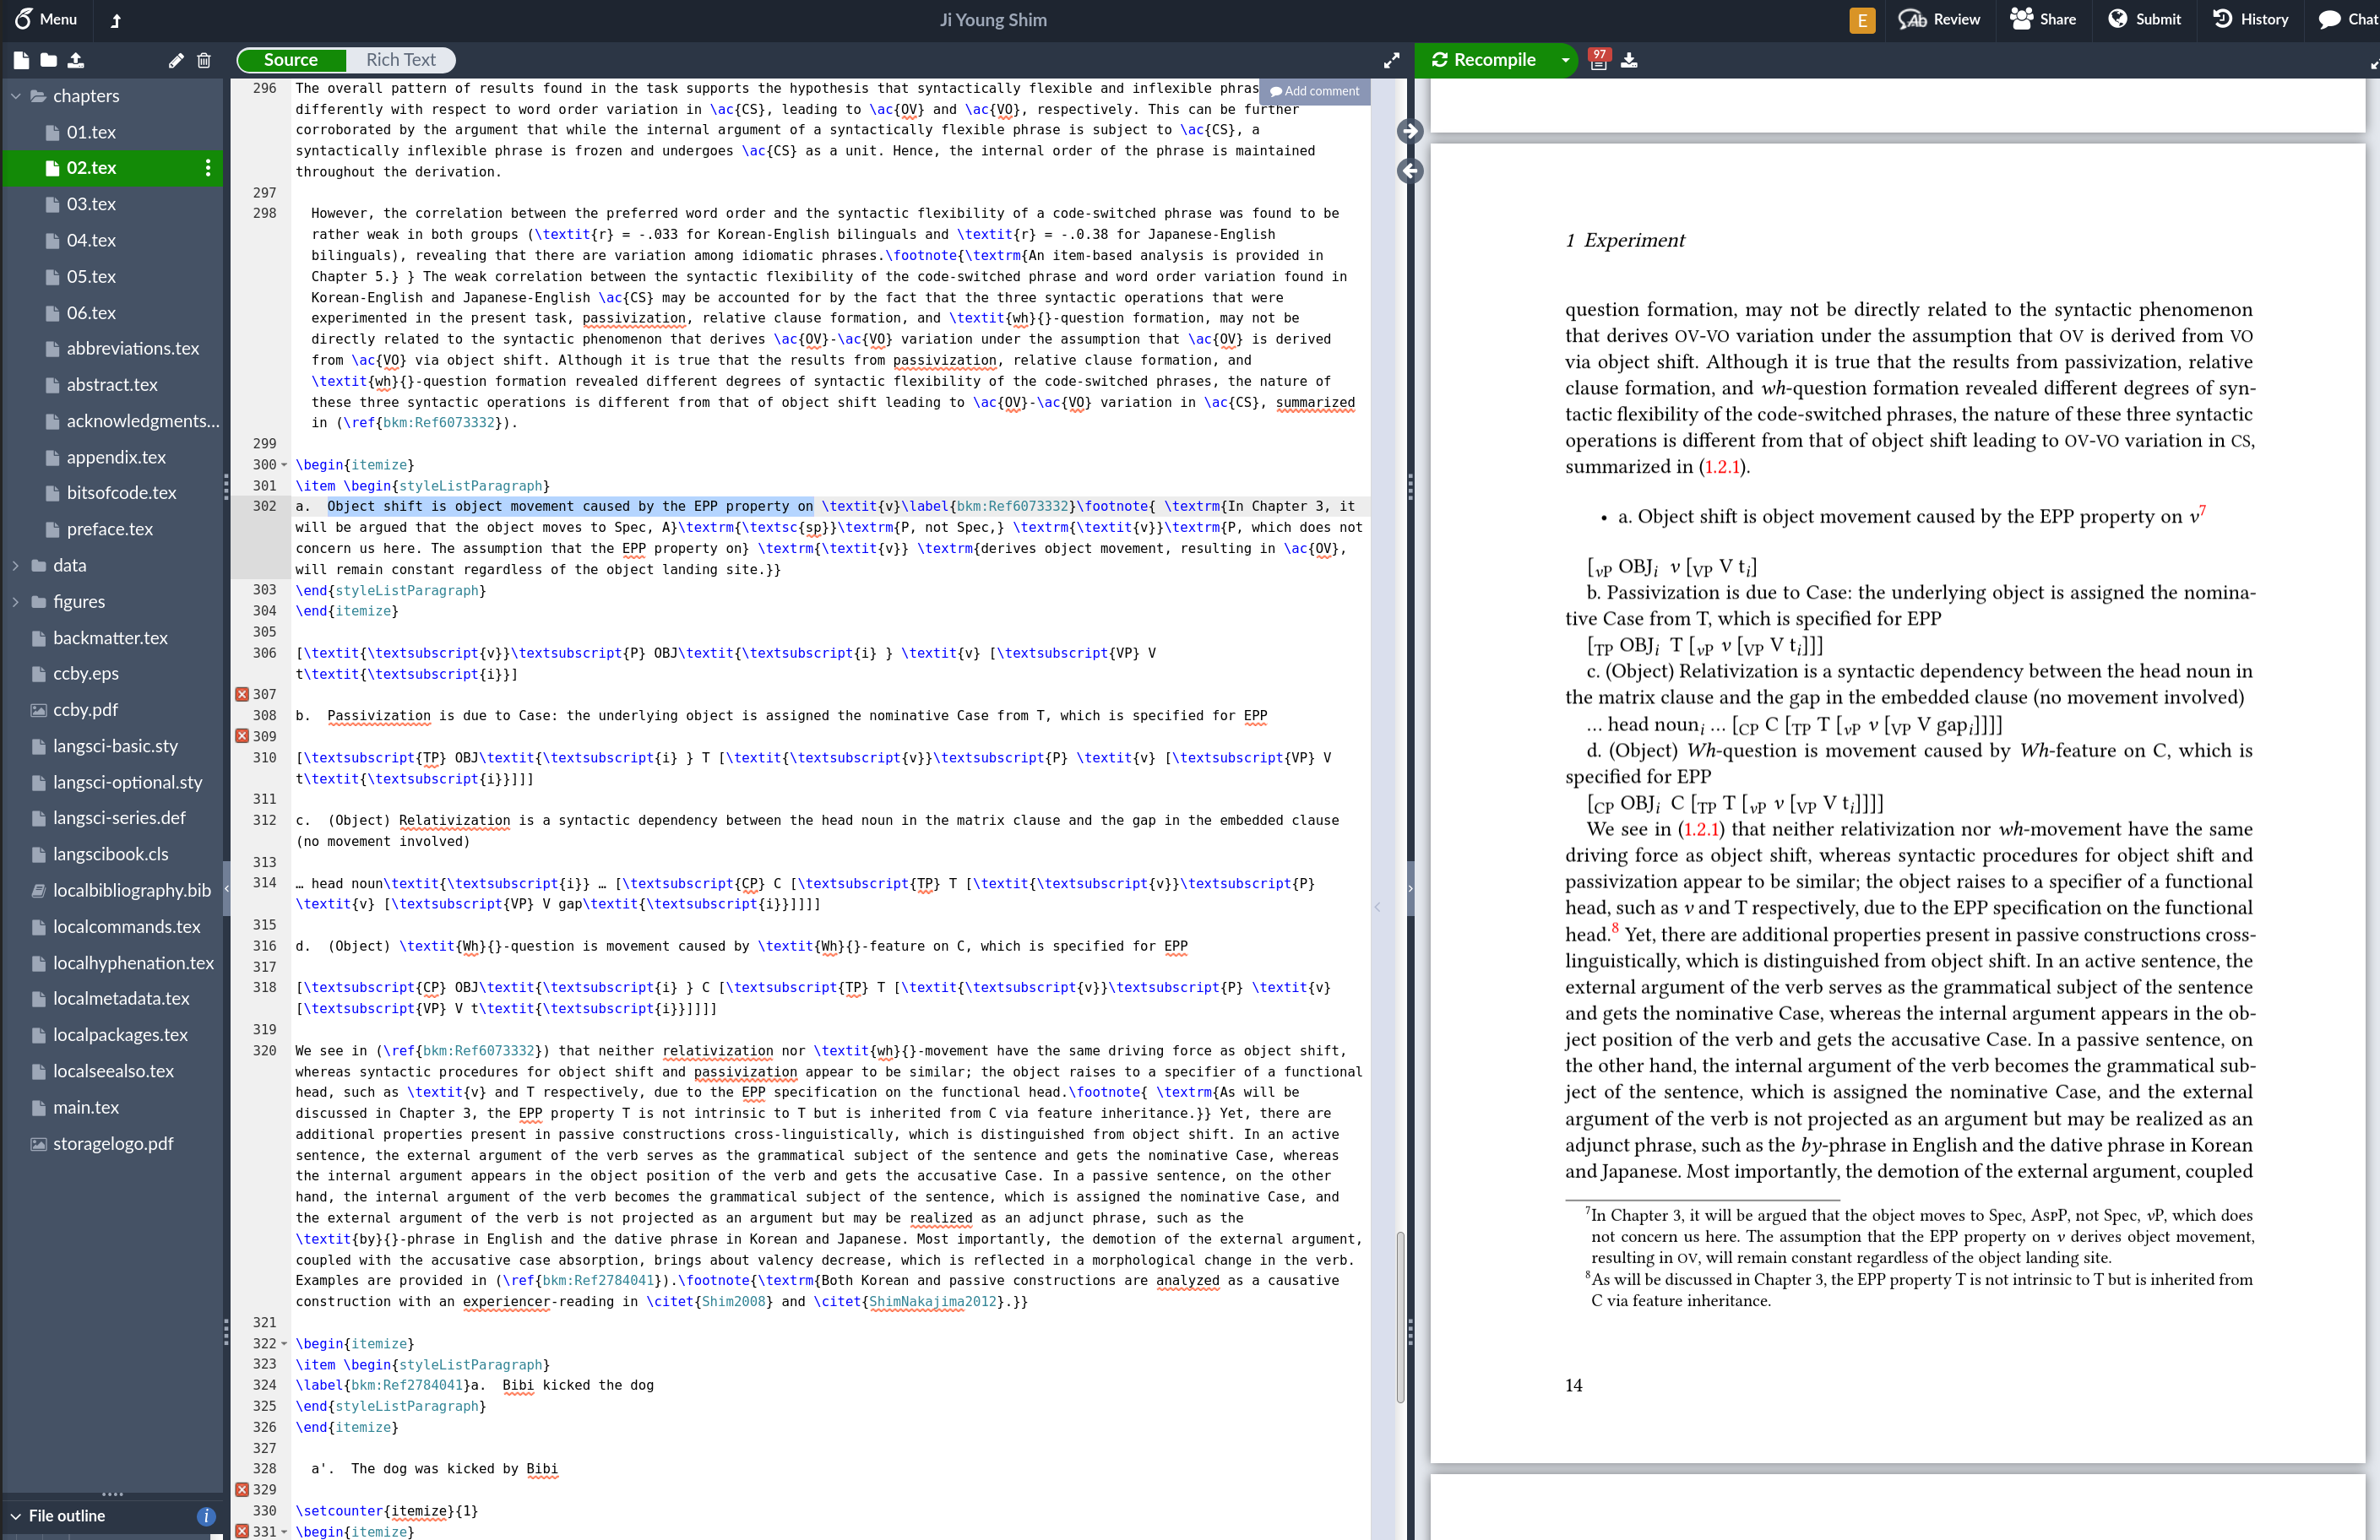
\includegraphics[width=1.1\textwidth]{overleaf2.png}
}

\frame{
\frametitle{Overleaf\newline collaborative approach}
%   \includegraphics[height=.2\textheight]{./path/to/graphicsfile}
  \begin{itemize}
    \item   we give one instance of a gold standard implementation for every given element type
    \item   replication is task for the author
    \item   we can possibly automatize some changes
    \item   interns etc can help as available
  \end{itemize}
}



\subsection{Edited volumes}

\frame{
\frametitle{Edited volumes}
\centering
 
\includegraphics[height=\textheight]{ACAL50.png}
}

\frame{
\frametitle{Edited volumes}
%   \includegraphics[height=.2\textheight]{./path/to/graphicsfile}
\begin{itemize}
  \item How to collect chapters?
  \begin{enumerate}
    \item email route
    \item online converter route
    \item expert route
  \end{enumerate}
\end{itemize}
}

\frame{
\frametitle{Email route}
%   \includegraphics[height=.2\textheight]{./path/to/graphicsfile}
  \begin{itemize}
   \item you send us the chapters as they are ready
   \begin{itemize}
     \item the more homogeneous the input, the more homogeneous the output
   \end{itemize}
   \item  we convert them and make the output available on Overleaf
   \begin{itemize}
     \item         file will compile
    \item         postprocessing will remain necessary
   \end{itemize}
    \item chapter conversion times to "look like an article with rough edges":
    \begin{itemize}
      \item
        uninitiated:
            hours to days
    \item
        LangSci:
            15--45 minutes
    \end{itemize}
  \end{itemize}
}


\frame{
\frametitle{Online converter route}
%   \includegraphics[height=.2\textheight]{./path/to/graphicsfile}
  \begin{itemize}
    \item
    editor collects chapters
   \item editor uses online converter
   \begin{itemize}
     \item \url{glottotopia.org/doc2tex/doc2tex}
   \end{itemize}

   \item chapters collected on Overleaf master project
   \item support available for tricky questions or dead ends
  \end{itemize}
}

% \frame{
% \frametitle{Online converter}
% %   \includegraphics[height=.2\textheight]{./path/to/graphicsfile}
%   \begin{itemize}
%     \item
%     \item
%   \end{itemize}
% }

\frame{
\frametitle{Overleaf: online converter}
\hspace*{-.5cm}\includegraphics[width=1.1\textwidth]{overleafwerner.png}
}

\frame{
\frametitle{Overleaf: online converter}
\hspace*{-.5cm}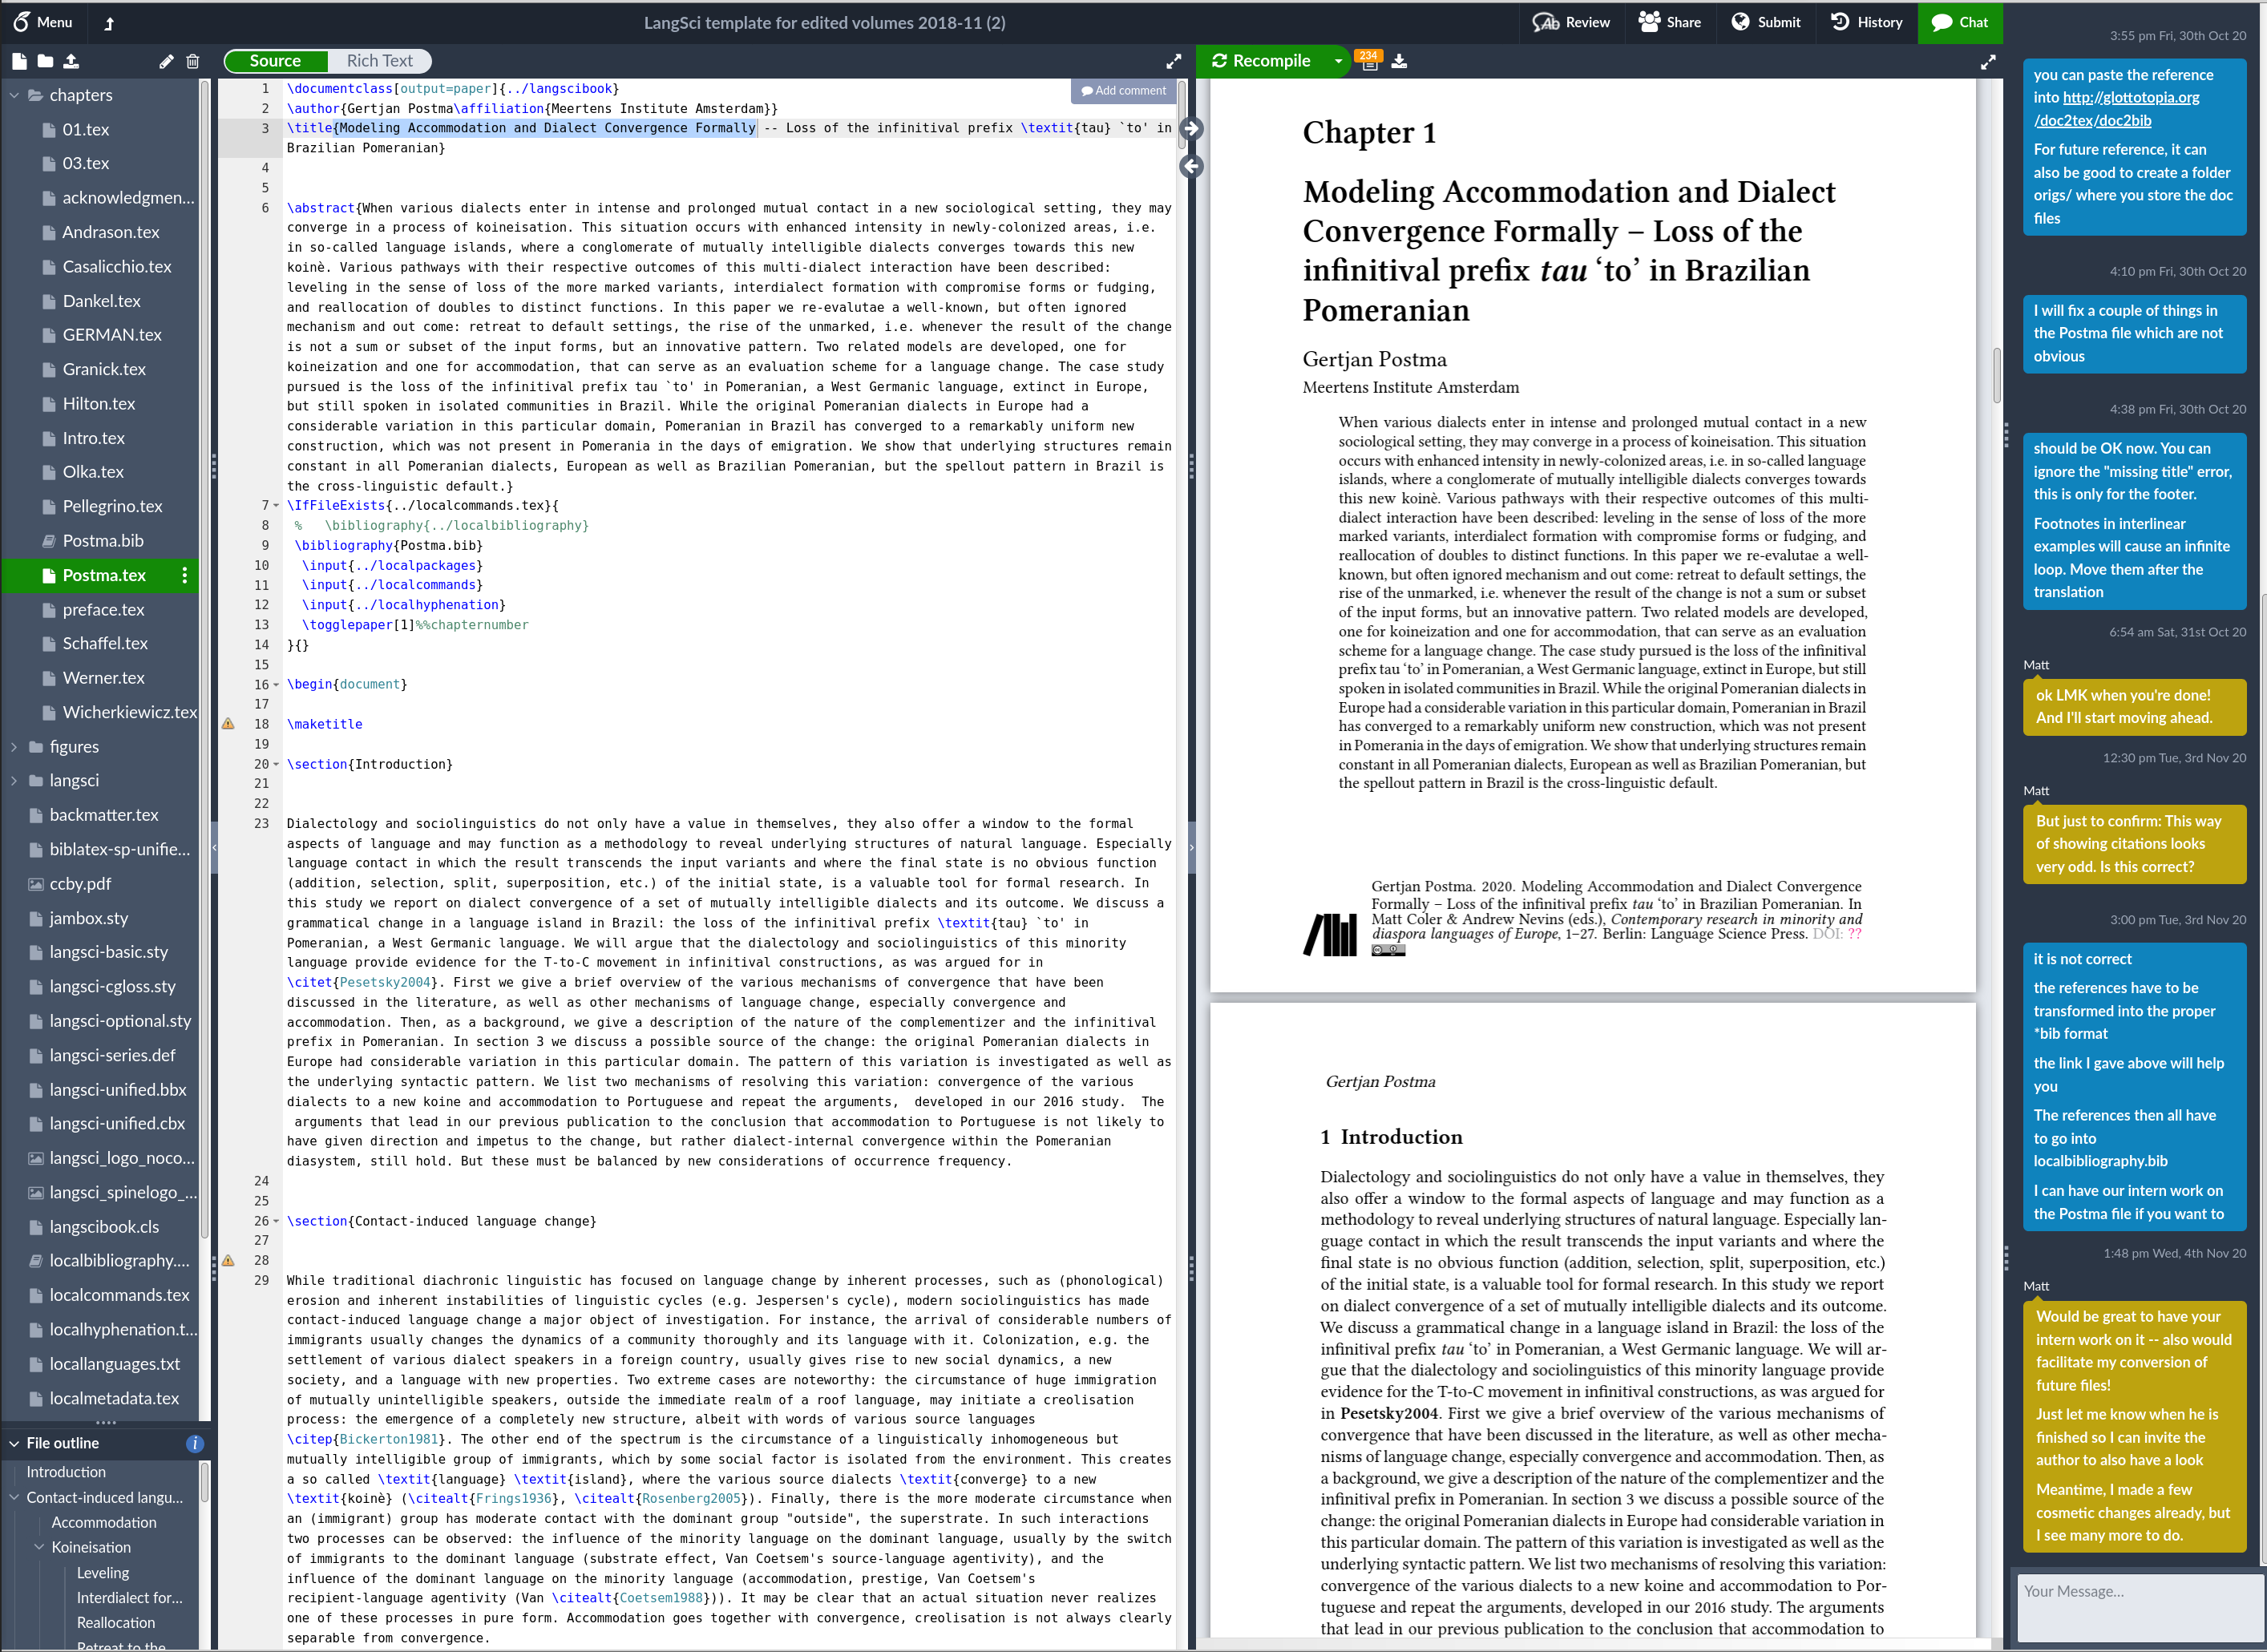
\includegraphics[width=1.1\textwidth]{overleafpostma.png}
}


\frame{
\frametitle{Expert route}
%   \includegraphics[height=.2\textheight]{./path/to/graphicsfile}
  \begin{itemize}
    \item  use offline conversion with \texttt{langsci} python package
    \item use sanity checker
    \item use GitHub
    \item even if the editors are experts they should allow LangSci to peek so we can see quickly when the project goes into the wrong direction
  \end{itemize}
}


\section{3 Golden Rules}
\frame{
\frametitle{3 rules for production}
  \begin{enumerate}
    \item \textbf{Early Bird Rule}
    \item  \textbf{Body Positivity Rule}
    \item  \textbf{Five Minute Rule}
  \end{enumerate}
}

\frame{
\frametitle{Early Bird Rule}
  \begin{itemize}
    \item {\LARGE   The answer to ``is it too early to show my manuscript to LangSci?'''is always ``No''.}
  \end{itemize}
}

\frame{
\frametitle{Body Positivity Rule}

\includegraphics[height=.3\textwidth]{photoshop1.jpg}~\pause

\includegraphics[height=.3\textwidth]{photoshop2.jpg}\pause
  \begin{itemize}
    \item {\large  Don't believe that people in magazines have perfect bodies. They don't.}
    \item {\large  Don't believe that other people's manuscripts are perfect. They aren't.}
    \item {\large  Do show us your code with all its imperfections.}
  \end{itemize}
}


\frame{
\frametitle{Five Minute Rule}
  \begin{itemize}
    \item {\LARGE   Authors should not spend more than 5 minutes trying to understand a LaTeX problem}
    \item Upon thinking/researching 5 minutes without finding the cause, please contact support@langsci-press.org.
    \item This will be faster for everybody.
  \end{itemize}
}

\section{Images}
\frame{
\frametitle{Production: images}
%   \includegraphics[height=.2\textheight]{./path/to/graphicsfile}
  \begin{itemize}
    \item  As a rule of thumb, we will recreate all images which are
    \begin{itemize}
      \item bar plots
      \item line plots
      \item classifications
      \item flow charts, semantic maps and the like
      \item maps
    \end{itemize}
    \item there are cases where this is not necessary, but they are rare
    \item R export is fine, preferably in pdf format.
    \item For screenshots, author should use the monitor with the most gigantic resolution they can find and maximize the relevant part.
  \end{itemize}
}



\end{document}
